\subsection{Dojo Funktion}


\subsection{Dojo Aufbau}
Das Design des Dojos aus Abbildung \ref{fig:DojoBild} wurde für die Batcherorarbeit von Jana Kalbermatten erarbeitet und dient als Vorlage für das Gerät. Der Dojo ist mit $245mm$ ziemlich lang, besitzt jedoch mit einem Aussendurchmesser von nur $19.5mm$ einen kleinen Querschnitt. Dieses Gehäuse setzt eine detailierte Planung der elektronischen Bauteile voraus, sowie ein kompaktes Design der elektronischen Schaltung.


\begin{figure}[h]
	\centering
	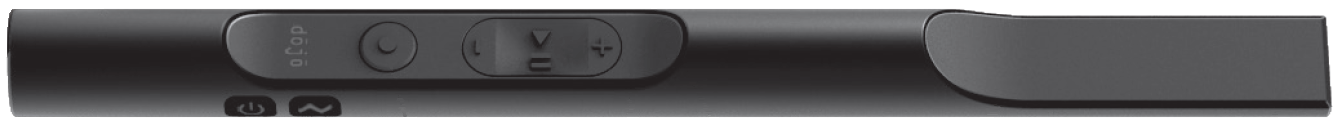
\includegraphics[width=\textwidth]{graphics/DojoBild.png}
	\caption{Aussenansicht des Dojos}
	\label{fig:DojoBild}
\end{figure}

Durch den begrenzten Durchmesser und der begrenzten Schiebeöffnung auf der Rückseite des Dojos kommen keine Akkumulatoren der Normgrösse $A$ sowie $AA$ infrage. Eingebaut wird daher ein Akkumulator der Grösse $AAA$. Um mit den Tastern und dem USB-Port nicht in konflikt zu geraten, wird der Akkumulator in der Mitte des Dojos eingebaut siehe Abbildung \ref{fig:DojoQuerschnitt}. Dies hat ebenfalls den Vorteil, das man einen Print der Länge $120mm$ einbauen kann, der den USB Port, sowie alle Taster beinhaltet.

\begin{figure}[h]
	\centering
	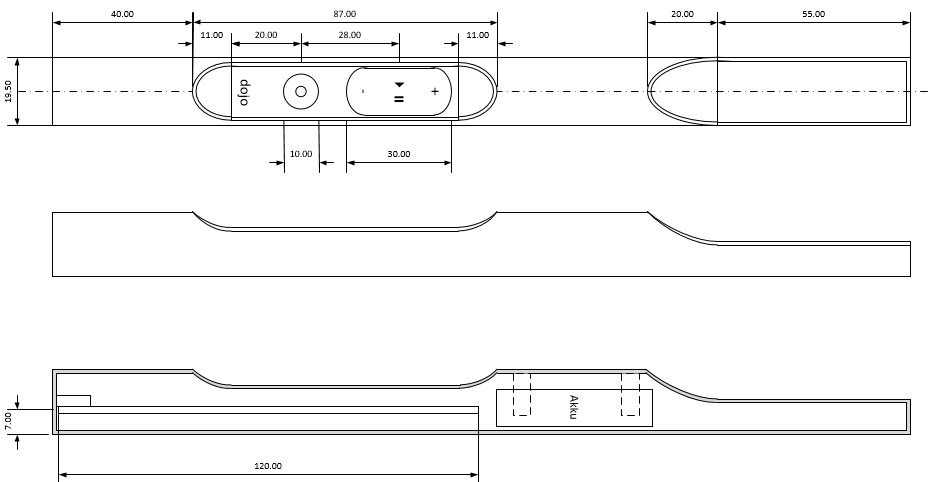
\includegraphics[width=\textwidth]{graphics/DojoQuerschnitt.png}
	\caption{Technische Zeichnung des Dojos}
	\label{fig:DojoQuerschnitt}
\end{figure}

\newpage

Der Akkumulator wird mit einer Stahl Batteriehalterung in das Gehäuse verbaut. Dabei bleibt, wie in der Abbildung \ref{fig:DojoAkkumulatorQuerschnitt} zu sehen, neben der Halterung genügend Platz für die Verbindungskabel, die zum Knochenschallgeber im Kopf des Dojos führen. Ebenfalls kann der Akkumulator durch den Schiebeöffner an der Rückseite des Dojos entfernt werden.

\begin{figure}[h]
	\centering
	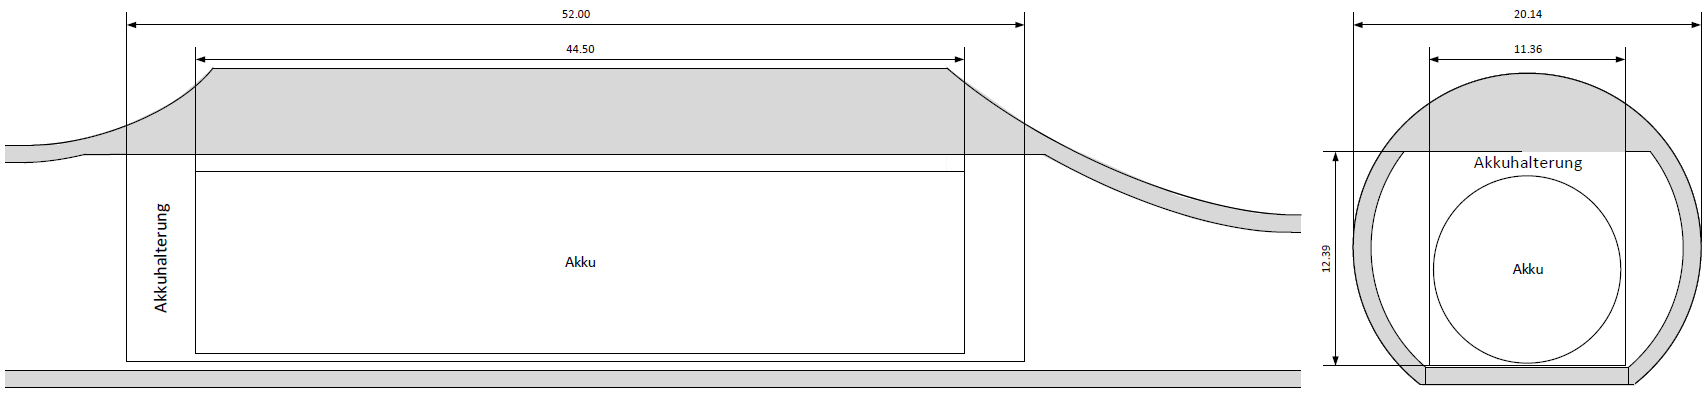
\includegraphics[width=\textwidth]{graphics/DojoAkkumulatorQuerschnitt.png}
	\caption{Positionierung des Akkumulators}
	\label{fig:DojoAkkumulatorQuerschnitt}
\end{figure}

Der Print nimmt mit einer Länge von $120mm$ und einer Breite von $17mm$ den grössten Teil des Gehäuses in Beschlag. Aufgrund der hohen Komplexität der elektronischen Schaltung handelt es sich um einen mehrlagigen Print. Am unteren Ende des Dojos befindet sich die Buchse der USB-Verbindung. Diese wird, wie in Abbildung \ref{fig:DojoPrintQuerschnitt} dargestellt, auf dem Print motiert. Die zweite Darstellung zeigt einen Querschnitt des Dojos bei den Tasten. Diese können auf dem Print montiert und mechanisch mit den Tastern des Gehäuses verbunden werden. Am Oberen Ende des Prints werden die Kontakte für die Batterie, sowie den Knochenschallgeber angebracht.

\begin{figure}[h]
	\centering
	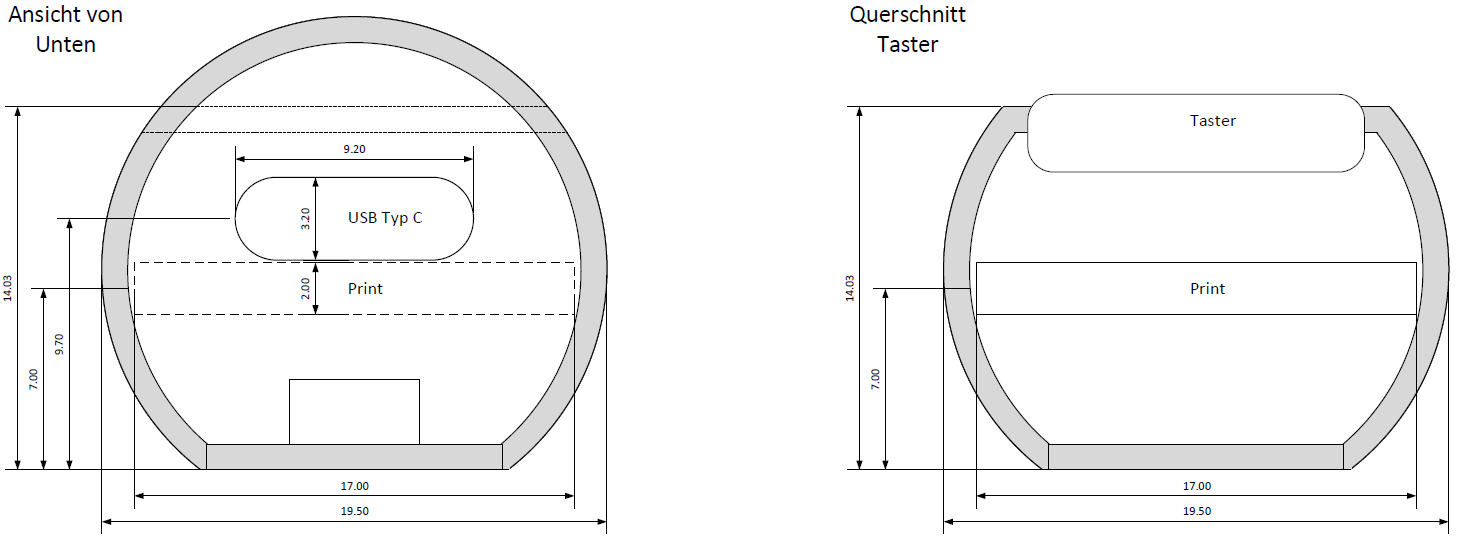
\includegraphics[width=\textwidth]{graphics/DojoPrintQuerschnitt.png}
	\caption{Positionierung des Prints}
	\label{fig:DojoPrintQuerschnitt}
\end{figure}

\newpage

\subsection{Technische Grundlagen}
